\documentclass[1p]{elsarticle_modified}
%\bibliographystyle{elsarticle-num}

%\usepackage[colorlinks]{hyperref}
%\usepackage{abbrmath_seonhwa} %\Abb, \Ascr, \Acal ,\Abf, \Afrak
\usepackage{amsfonts}
\usepackage{amssymb}
\usepackage{amsmath}
\usepackage{amsthm}
\usepackage{scalefnt}
\usepackage{amsbsy}
\usepackage{kotex}
\usepackage{caption}
\usepackage{subfig}
\usepackage{color}
\usepackage{graphicx}
\usepackage{xcolor} %% white, black, red, green, blue, cyan, magenta, yellow
\usepackage{float}
\usepackage{setspace}
\usepackage{hyperref}

\usepackage{tikz}
\usetikzlibrary{arrows}

\usepackage{multirow}
\usepackage{array} % fixed length table
\usepackage{hhline}

%%%%%%%%%%%%%%%%%%%%%
\makeatletter
\renewcommand*\env@matrix[1][\arraystretch]{%
	\edef\arraystretch{#1}%
	\hskip -\arraycolsep
	\let\@ifnextchar\new@ifnextchar
	\array{*\c@MaxMatrixCols c}}
\makeatother %https://tex.stackexchange.com/questions/14071/how-can-i-increase-the-line-spacing-in-a-matrix
%%%%%%%%%%%%%%%

\usepackage[normalem]{ulem}

\newcommand{\msout}[1]{\ifmmode\text{\sout{\ensuremath{#1}}}\else\sout{#1}\fi}
%SOURCE: \msout is \stkout macro in https://tex.stackexchange.com/questions/20609/strikeout-in-math-mode

\newcommand{\cancel}[1]{
	\ifmmode
	{\color{red}\msout{#1}}
	\else
	{\color{red}\sout{#1}}
	\fi
}

\newcommand{\add}[1]{
	{\color{blue}\uwave{#1}}
}

\newcommand{\replace}[2]{
	\ifmmode
	{\color{red}\msout{#1}}{\color{blue}\uwave{#2}}
	\else
	{\color{red}\sout{#1}}{\color{blue}\uwave{#2}}
	\fi
}

\newcommand{\Sol}{\mathcal{S}} %segment
\newcommand{\D}{D} %diagram
\newcommand{\A}{\mathcal{A}} %arc


%%%%%%%%%%%%%%%%%%%%%%%%%%%%%5 test

\def\sl{\operatorname{\textup{SL}}(2,\Cbb)}
\def\psl{\operatorname{\textup{PSL}}(2,\Cbb)}
\def\quan{\mkern 1mu \triangleright \mkern 1mu}

\theoremstyle{definition}
\newtheorem{thm}{Theorem}[section]
\newtheorem{prop}[thm]{Proposition}
\newtheorem{lem}[thm]{Lemma}
\newtheorem{ques}[thm]{Question}
\newtheorem{cor}[thm]{Corollary}
\newtheorem{defn}[thm]{Definition}
\newtheorem{exam}[thm]{Example}
\newtheorem{rmk}[thm]{Remark}
\newtheorem{alg}[thm]{Algorithm}

\newcommand{\I}{\sqrt{-1}}
\begin{document}

%\begin{frontmatter}
%
%\title{Boundary parabolic representations of knots up to 8 crossings}
%
%%% Group authors per affiliation:
%\author{Yunhi Cho} 
%\address{Department of Mathematics, University of Seoul, Seoul, Korea}
%\ead{yhcho@uos.ac.kr}
%
%
%\author{Seonhwa Kim} %\fnref{s_kim}}
%\address{Center for Geometry and Physics, Institute for Basic Science, Pohang, 37673, Korea}
%\ead{ryeona17@ibs.re.kr}
%
%\author{Hyuk Kim}
%\address{Department of Mathematical Sciences, Seoul National University, Seoul 08826, Korea}
%\ead{hyukkim@snu.ac.kr}
%
%\author{Seokbeom Yoon}
%\address{Department of Mathematical Sciences, Seoul National University, Seoul, 08826,  Korea}
%\ead{sbyoon15@snu.ac.kr}
%
%\begin{abstract}
%We find all boundary parabolic representation of knots up to 8 crossings.
%
%\end{abstract}
%\begin{keyword}
%    \MSC[2010] 57M25 
%\end{keyword}
%
%\end{frontmatter}

%\linenumbers
%\tableofcontents
%
\newcommand\colored[1]{\textcolor{white}{\rule[-0.35ex]{0.8em}{1.4ex}}\kern-0.8em\color{red} #1}%
%\newcommand\colored[1]{\textcolor{white}{ #1}\kern-2.17ex	\textcolor{white}{ #1}\kern-1.81ex	\textcolor{white}{ #1}\kern-2.15ex\color{red}#1	}

{\Large $\underline{12a_{1233}~(K12a_{1233})}$}

\setlength{\tabcolsep}{10pt}
\renewcommand{\arraystretch}{1.6}
\vspace{1cm}\begin{tabular}{m{100pt}>{\centering\arraybackslash}m{274pt}}
\multirow{5}{120pt}{
	\centering
	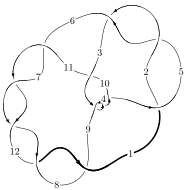
\includegraphics[width=112pt]{../../../GIT/diagram.site/Diagrams/png/2034_12a_1233.png}\\
\ \ \ A knot diagram\footnotemark}&
\allowdisplaybreaks
\textbf{Linearized knot diagam} \\
\cline{2-2}
 &
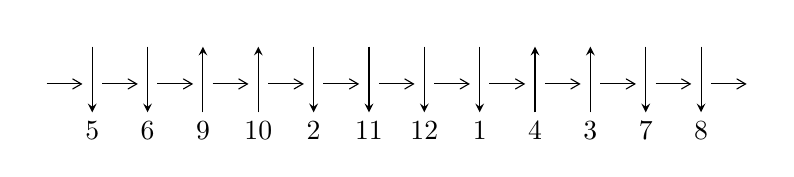
\begin{tikzpicture}[x=20pt, y=17pt]
	% nodes
	\node (C0) at (0, 0) {};
	\node (C1) at (1, 0) {};
	\node (C1U) at (1, +1) {};
	\node (C1D) at (1, -1) {5};

	\node (C2) at (2, 0) {};
	\node (C2U) at (2, +1) {};
	\node (C2D) at (2, -1) {6};

	\node (C3) at (3, 0) {};
	\node (C3U) at (3, +1) {};
	\node (C3D) at (3, -1) {9};

	\node (C4) at (4, 0) {};
	\node (C4U) at (4, +1) {};
	\node (C4D) at (4, -1) {10};

	\node (C5) at (5, 0) {};
	\node (C5U) at (5, +1) {};
	\node (C5D) at (5, -1) {2};

	\node (C6) at (6, 0) {};
	\node (C6U) at (6, +1) {};
	\node (C6D) at (6, -1) {11};

	\node (C7) at (7, 0) {};
	\node (C7U) at (7, +1) {};
	\node (C7D) at (7, -1) {12};

	\node (C8) at (8, 0) {};
	\node (C8U) at (8, +1) {};
	\node (C8D) at (8, -1) {1};

	\node (C9) at (9, 0) {};
	\node (C9U) at (9, +1) {};
	\node (C9D) at (9, -1) {4};

	\node (C10) at (10, 0) {};
	\node (C10U) at (10, +1) {};
	\node (C10D) at (10, -1) {3};

	\node (C11) at (11, 0) {};
	\node (C11U) at (11, +1) {};
	\node (C11D) at (11, -1) {7};

	\node (C12) at (12, 0) {};
	\node (C12U) at (12, +1) {};
	\node (C12D) at (12, -1) {8};
	\node (C13) at (13, 0) {};

	% arrows
	\draw[->,>={angle 60}]
	(C0) edge (C1) (C1) edge (C2) (C2) edge (C3) (C3) edge (C4) (C4) edge (C5) (C5) edge (C6) (C6) edge (C7) (C7) edge (C8) (C8) edge (C9) (C9) edge (C10) (C10) edge (C11) (C11) edge (C12) (C12) edge (C13) ;	\draw[->,>=stealth]
	(C1U) edge (C1D) (C2U) edge (C2D) (C3D) edge (C3U) (C4D) edge (C4U) (C5U) edge (C5D) (C6U) edge (C6D) (C7U) edge (C7D) (C8U) edge (C8D) (C9D) edge (C9U) (C10D) edge (C10U) (C11U) edge (C11D) (C12U) edge (C12D) ;
	\end{tikzpicture} \\
\hhline{~~} \\& 
\textbf{Solving Sequence} \\ \cline{2-2} 
 &
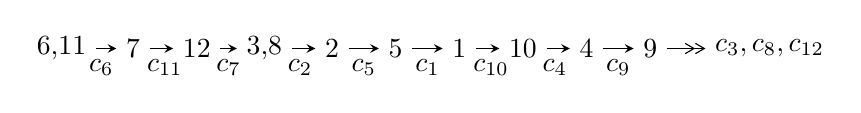
\begin{tikzpicture}[x=23pt, y=7pt]
	% node
	\node (A0) at (-1/8, 0) {6,11};
	\node (A1) at (1, 0) {7};
	\node (A2) at (2, 0) {12};
	\node (A3) at (49/16, 0) {3,8};
	\node (A4) at (33/8, 0) {2};
	\node (A5) at (41/8, 0) {5};
	\node (A6) at (49/8, 0) {1};
	\node (A7) at (57/8, 0) {10};
	\node (A8) at (65/8, 0) {4};
	\node (A9) at (73/8, 0) {9};
	\node (C1) at (1/2, -1) {$c_{6}$};
	\node (C2) at (3/2, -1) {$c_{11}$};
	\node (C3) at (5/2, -1) {$c_{7}$};
	\node (C4) at (29/8, -1) {$c_{2}$};
	\node (C5) at (37/8, -1) {$c_{5}$};
	\node (C6) at (45/8, -1) {$c_{1}$};
	\node (C7) at (53/8, -1) {$c_{10}$};
	\node (C8) at (61/8, -1) {$c_{4}$};
	\node (C9) at (69/8, -1) {$c_{9}$};
	\node (A10) at (11, 0) {$c_{3},c_{8},c_{12}$};

	% edge
	\draw[->,>=stealth]	
	(A0) edge (A1) (A1) edge (A2) (A2) edge (A3) (A3) edge (A4) (A4) edge (A5) (A5) edge (A6) (A6) edge (A7) (A7) edge (A8) (A8) edge (A9) ;
	\draw[->>,>={angle 60}]	
	(A9) edge (A10);
\end{tikzpicture} \\ 

\end{tabular} \\

\footnotetext{
The image of knot diagram is generated by the software ``\textbf{Draw programme}" developed by Andrew Bartholomew(\url{http://www.layer8.co.uk/maths/draw/index.htm\#Running-draw}), where we modified some parts for our purpose(\url{https://github.com/CATsTAILs/LinksPainter}).
}\phantom \\ \newline 
\centering \textbf{Ideals for irreducible components\footnotemark of $X_{\text{par}}$} 
 
\begin{align*}
I^u_{1}&=\langle 
55915836184337 u^{43}+64179161931292 u^{42}+\cdots+45302578214423 b+117930377236025,\\
\phantom{I^u_{1}}&\phantom{= \langle  }-212034836392771 u^{43}-365740891628043 u^{42}+\cdots+90605156428846 a-1349574182090028,\\
\phantom{I^u_{1}}&\phantom{= \langle  }u^{44}+2 u^{43}+\cdots+10 u+1\rangle \\
I^u_{2}&=\langle 
b+1,\;a,\;u^2+u-1\rangle \\
I^u_{3}&=\langle 
b-1,\;a^2+2 u-4,\;u^2- u-1\rangle \\
\\
\end{align*}
\raggedright * 3 irreducible components of $\dim_{\mathbb{C}}=0$, with total 50 representations.\\
\footnotetext{All coefficients of polynomials are rational numbers. But the coefficients are sometimes approximated in decimal forms when there is not enough margin.}
\newpage
\renewcommand{\arraystretch}{1}
\centering \section*{I. $I^u_{1}= \langle 5.59\times10^{13} u^{43}+6.42\times10^{13} u^{42}+\cdots+4.53\times10^{13} b+1.18\times10^{14},\;-2.12\times10^{14} u^{43}-3.66\times10^{14} u^{42}+\cdots+9.06\times10^{13} a-1.35\times10^{15},\;u^{44}+2 u^{43}+\cdots+10 u+1 \rangle$}
\flushleft \textbf{(i) Arc colorings}\\
\begin{tabular}{m{7pt} m{180pt} m{7pt} m{180pt} }
\flushright $a_{6}=$&$\begin{pmatrix}1\\0\end{pmatrix}$ \\
\flushright $a_{11}=$&$\begin{pmatrix}0\\u\end{pmatrix}$ \\
\flushright $a_{7}=$&$\begin{pmatrix}1\\u^2\end{pmatrix}$ \\
\flushright $a_{12}=$&$\begin{pmatrix}- u\\- u^3+u\end{pmatrix}$ \\
\flushright $a_{3}=$&$\begin{pmatrix}2.34021 u^{43}+4.03665 u^{42}+\cdots+34.7587 u+14.8951\\-1.23427 u^{43}-1.41668 u^{42}+\cdots-12.4742 u-2.60317\end{pmatrix}$ \\
\flushright $a_{8}=$&$\begin{pmatrix}- u^2+1\\- u^4+2 u^2\end{pmatrix}$ \\
\flushright $a_{2}=$&$\begin{pmatrix}1.10593 u^{43}+2.61997 u^{42}+\cdots+22.2845 u+12.2919\\-1.23427 u^{43}-1.41668 u^{42}+\cdots-12.4742 u-2.60317\end{pmatrix}$ \\
\flushright $a_{5}=$&$\begin{pmatrix}1.85429 u^{43}+3.86193 u^{42}+\cdots+41.9220 u+15.2508\\-0.560033 u^{43}-0.357346 u^{42}+\cdots+0.835350 u-0.740724\end{pmatrix}$ \\
\flushright $a_{1}=$&$\begin{pmatrix}u^3-2 u\\u^5-3 u^3+u\end{pmatrix}$ \\
\flushright $a_{10}=$&$\begin{pmatrix}2.83815 u^{43}+5.23204 u^{42}+\cdots+53.7766 u+20.3839\\-0.609358 u^{43}-0.379534 u^{42}+\cdots-8.15167 u-2.41432\end{pmatrix}$ \\
\flushright $a_{4}=$&$\begin{pmatrix}-1.91530 u^{43}-3.28109 u^{42}+\cdots-28.9627 u-12.6975\\0.723413 u^{43}+1.18474 u^{42}+\cdots+12.5122 u+2.70679\end{pmatrix}$ \\
\flushright $a_{9}=$&$\begin{pmatrix}u^4-3 u^2+1\\u^6-4 u^4+3 u^2\end{pmatrix}$\\&\end{tabular}
\flushleft \textbf{(ii) Obstruction class $= -1$}\\~\\
\flushleft \textbf{(iii) Cusp Shapes $= -\frac{18072105995455}{45302578214423} u^{43}-\frac{25950739447177}{45302578214423} u^{42}+\cdots-\frac{71920607974749}{45302578214423} u+\frac{76480599133623}{45302578214423}$}\\~\\
\newpage\renewcommand{\arraystretch}{1}
\flushleft \textbf{(iv) u-Polynomials at the component}\newline \\
\begin{tabular}{m{50pt}|m{274pt}}
Crossings & \hspace{64pt}u-Polynomials at each crossing \\
\hline $$\begin{aligned}c_{1},c_{2},c_{5}\end{aligned}$$&$\begin{aligned}
&u^{44}+3 u^{43}+\cdots-11 u-1
\end{aligned}$\\
\hline $$\begin{aligned}c_{3},c_{4},c_{9}\end{aligned}$$&$\begin{aligned}
&u^{44}- u^{43}+\cdots+4 u+4
\end{aligned}$\\
\hline $$\begin{aligned}c_{6},c_{7},c_{8}\\c_{11},c_{12}\end{aligned}$$&$\begin{aligned}
&u^{44}-2 u^{43}+\cdots-10 u+1
\end{aligned}$\\
\hline $$\begin{aligned}c_{10}\end{aligned}$$&$\begin{aligned}
&u^{44}+3 u^{43}+\cdots-540 u-68
\end{aligned}$\\
\hline
\end{tabular}\\~\\
\newpage\renewcommand{\arraystretch}{1}
\flushleft \textbf{(v) Riley Polynomials at the component}\newline \\
\begin{tabular}{m{50pt}|m{274pt}}
Crossings & \hspace{64pt}Riley Polynomials at each crossing \\
\hline $$\begin{aligned}c_{1},c_{2},c_{5}\end{aligned}$$&$\begin{aligned}
&y^{44}-45 y^{43}+\cdots-251 y+1
\end{aligned}$\\
\hline $$\begin{aligned}c_{3},c_{4},c_{9}\end{aligned}$$&$\begin{aligned}
&y^{44}-39 y^{43}+\cdots-176 y+16
\end{aligned}$\\
\hline $$\begin{aligned}c_{6},c_{7},c_{8}\\c_{11},c_{12}\end{aligned}$$&$\begin{aligned}
&y^{44}-60 y^{43}+\cdots-66 y+1
\end{aligned}$\\
\hline $$\begin{aligned}c_{10}\end{aligned}$$&$\begin{aligned}
&y^{44}+21 y^{43}+\cdots-261680 y+4624
\end{aligned}$\\
\hline
\end{tabular}\\~\\
\newpage\flushleft \textbf{(vi) Complex Volumes and Cusp Shapes}
$$\begin{array}{c|c|c}  
\text{Solutions to }I^u_{1}& \I (\text{vol} + \sqrt{-1}CS) & \text{Cusp shape}\\
 \hline 
\begin{aligned}
u &= \phantom{-}0.998544 + 0.111218 I \\
a &= \phantom{-}0.351759 - 0.614033 I \\
b &= -0.801508 + 0.547302 I\end{aligned}
 & -0.663058 - 0.817762 I & -8.32759 + 0.71545 I \\ \hline\begin{aligned}
u &= \phantom{-}0.998544 - 0.111218 I \\
a &= \phantom{-}0.351759 + 0.614033 I \\
b &= -0.801508 - 0.547302 I\end{aligned}
 & -0.663058 + 0.817762 I & -8.32759 - 0.71545 I \\ \hline\begin{aligned}
u &= -1.001850 + 0.127057 I \\
a &= \phantom{-}0.120314 + 0.945722 I \\
b &= \phantom{-}0.516618 - 0.643752 I\end{aligned}
 & -3.83529 + 2.20768 I & -11.83990 - 4.73522 I \\ \hline\begin{aligned}
u &= -1.001850 - 0.127057 I \\
a &= \phantom{-}0.120314 - 0.945722 I \\
b &= \phantom{-}0.516618 + 0.643752 I\end{aligned}
 & -3.83529 - 2.20768 I & -11.83990 + 4.73522 I \\ \hline\begin{aligned}
u &= -0.954649\phantom{ +0.000000I} \\
a &= -2.19836\phantom{ +0.000000I} \\
b &= -1.29146\phantom{ +0.000000I}\end{aligned}
 & \phantom{-}0.461481\phantom{ +0.000000I} & -10.4800\phantom{ +0.000000I} \\ \hline\begin{aligned}
u &= \phantom{-}1.009480 + 0.273056 I \\
a &= -0.335081 + 1.217640 I \\
b &= -0.390450 - 0.804941 I\end{aligned}
 & \phantom{-}0.61880 - 5.62694 I & -5.80251 + 6.42762 I \\ \hline\begin{aligned}
u &= \phantom{-}1.009480 - 0.273056 I \\
a &= -0.335081 - 1.217640 I \\
b &= -0.390450 + 0.804941 I\end{aligned}
 & \phantom{-}0.61880 + 5.62694 I & -5.80251 - 6.42762 I \\ \hline\begin{aligned}
u &= \phantom{-}1.065250 + 0.397438 I \\
a &= \phantom{-}0.04875 - 1.63500 I \\
b &= \phantom{-}1.49141 + 0.28927 I\end{aligned}
 & -5.49263 - 9.59429 I & -8.85592 + 6.59284 I \\ \hline\begin{aligned}
u &= \phantom{-}1.065250 - 0.397438 I \\
a &= \phantom{-}0.04875 + 1.63500 I \\
b &= \phantom{-}1.49141 - 0.28927 I\end{aligned}
 & -5.49263 + 9.59429 I & -8.85592 - 6.59284 I \\ \hline\begin{aligned}
u &= -1.131940 + 0.326750 I \\
a &= -0.162725 - 1.267720 I \\
b &= -1.50777 + 0.18978 I\end{aligned}
 & -10.46760 + 5.17349 I & -13.11043 - 4.56372 I\\
 \hline 
 \end{array}$$\newpage$$\begin{array}{c|c|c}  
\text{Solutions to }I^u_{1}& \I (\text{vol} + \sqrt{-1}CS) & \text{Cusp shape}\\
 \hline 
\begin{aligned}
u &= -1.131940 - 0.326750 I \\
a &= -0.162725 + 1.267720 I \\
b &= -1.50777 - 0.18978 I\end{aligned}
 & -10.46760 - 5.17349 I & -13.11043 + 4.56372 I \\ \hline\begin{aligned}
u &= \phantom{-}1.193530 + 0.183455 I \\
a &= \phantom{-}0.388564 - 0.688390 I \\
b &= \phantom{-}1.47060 + 0.06865 I\end{aligned}
 & -7.96364 - 0.55193 I & -10.90446 + 0. I\phantom{ +0.000000I} \\ \hline\begin{aligned}
u &= \phantom{-}1.193530 - 0.183455 I \\
a &= \phantom{-}0.388564 + 0.688390 I \\
b &= \phantom{-}1.47060 - 0.06865 I\end{aligned}
 & -7.96364 + 0.55193 I & -10.90446 + 0. I\phantom{ +0.000000I} \\ \hline\begin{aligned}
u &= -0.534767 + 0.564063 I \\
a &= -1.168730 + 0.715602 I \\
b &= \phantom{-}1.42904 + 0.11240 I\end{aligned}
 & -2.23516 - 1.94324 I & -7.08189 - 0.05666 I \\ \hline\begin{aligned}
u &= -0.534767 - 0.564063 I \\
a &= -1.168730 - 0.715602 I \\
b &= \phantom{-}1.42904 - 0.11240 I\end{aligned}
 & -2.23516 + 1.94324 I & -7.08189 + 0.05666 I \\ \hline\begin{aligned}
u &= \phantom{-}0.767069\phantom{ +0.000000I} \\
a &= -0.450820\phantom{ +0.000000I} \\
b &= -0.373478\phantom{ +0.000000I}\end{aligned}
 & -1.47485\phantom{ +0.000000I} & -4.57540\phantom{ +0.000000I} \\ \hline\begin{aligned}
u &= \phantom{-}0.374316 + 0.607175 I \\
a &= \phantom{-}1.31959 + 1.13185 I \\
b &= -1.43997 - 0.06548 I\end{aligned}
 & -5.73016 - 1.98434 I & -10.23333 + 3.59268 I \\ \hline\begin{aligned}
u &= \phantom{-}0.374316 - 0.607175 I \\
a &= \phantom{-}1.31959 - 1.13185 I \\
b &= -1.43997 + 0.06548 I\end{aligned}
 & -5.73016 + 1.98434 I & -10.23333 - 3.59268 I \\ \hline\begin{aligned}
u &= -0.257658 + 0.663265 I \\
a &= -1.53428 + 1.37125 I \\
b &= \phantom{-}1.44829 - 0.20795 I\end{aligned}
 & -1.39014 + 5.99441 I & -5.18773 - 5.53945 I \\ \hline\begin{aligned}
u &= -0.257658 - 0.663265 I \\
a &= -1.53428 - 1.37125 I \\
b &= \phantom{-}1.44829 + 0.20795 I\end{aligned}
 & -1.39014 - 5.99441 I & -5.18773 + 5.53945 I\\
 \hline 
 \end{array}$$\newpage$$\begin{array}{c|c|c}  
\text{Solutions to }I^u_{1}& \I (\text{vol} + \sqrt{-1}CS) & \text{Cusp shape}\\
 \hline 
\begin{aligned}
u &= -0.475748 + 0.282175 I \\
a &= \phantom{-}1.74537 + 0.58249 I \\
b &= -0.390691 - 0.314994 I\end{aligned}
 & \phantom{-}3.52033 - 0.22404 I & -1.41771 - 1.59086 I \\ \hline\begin{aligned}
u &= -0.475748 - 0.282175 I \\
a &= \phantom{-}1.74537 - 0.58249 I \\
b &= -0.390691 + 0.314994 I\end{aligned}
 & \phantom{-}3.52033 + 0.22404 I & -1.41771 + 1.59086 I \\ \hline\begin{aligned}
u &= -0.209850 + 0.494994 I \\
a &= \phantom{-}0.58968 - 2.01314 I \\
b &= -0.337217 + 0.618314 I\end{aligned}
 & \phantom{-}4.39585 + 3.01078 I & \phantom{-}0.72066 - 6.01437 I \\ \hline\begin{aligned}
u &= -0.209850 - 0.494994 I \\
a &= \phantom{-}0.58968 + 2.01314 I \\
b &= -0.337217 - 0.618314 I\end{aligned}
 & \phantom{-}4.39585 - 3.01078 I & \phantom{-}0.72066 + 6.01437 I \\ \hline\begin{aligned}
u &= \phantom{-}1.50823\phantom{ +0.000000I} \\
a &= -0.100172\phantom{ +0.000000I} \\
b &= \phantom{-}1.32001\phantom{ +0.000000I}\end{aligned}
 & -8.29422\phantom{ +0.000000I} & \phantom{-0.000000 } 0 \\ \hline\begin{aligned}
u &= -0.387467\phantom{ +0.000000I} \\
a &= \phantom{-}0.781408\phantom{ +0.000000I} \\
b &= \phantom{-}1.09644\phantom{ +0.000000I}\end{aligned}
 & -2.22865\phantom{ +0.000000I} & \phantom{-}3.06750\phantom{ +0.000000I} \\ \hline\begin{aligned}
u &= \phantom{-}1.62350\phantom{ +0.000000I} \\
a &= \phantom{-}0.906030\phantom{ +0.000000I} \\
b &= \phantom{-}0.0651186\phantom{ +0.000000I}\end{aligned}
 & -3.95658\phantom{ +0.000000I} & \phantom{-0.000000 } 0 \\ \hline\begin{aligned}
u &= -1.64624\phantom{ +0.000000I} \\
a &= -0.216085\phantom{ +0.000000I} \\
b &= -0.708554\phantom{ +0.000000I}\end{aligned}
 & -9.99566\phantom{ +0.000000I} & \phantom{-0.000000 } 0 \\ \hline\begin{aligned}
u &= \phantom{-}0.189239 + 0.289124 I \\
a &= -0.78500 - 1.22940 I \\
b &= \phantom{-}0.260740 + 0.297980 I\end{aligned}
 & -0.172531 - 0.795475 I & -4.76256 + 8.61865 I \\ \hline\begin{aligned}
u &= \phantom{-}0.189239 - 0.289124 I \\
a &= -0.78500 + 1.22940 I \\
b &= \phantom{-}0.260740 - 0.297980 I\end{aligned}
 & -0.172531 + 0.795475 I & -4.76256 - 8.61865 I\\
 \hline 
 \end{array}$$\newpage$$\begin{array}{c|c|c}  
\text{Solutions to }I^u_{1}& \I (\text{vol} + \sqrt{-1}CS) & \text{Cusp shape}\\
 \hline 
\begin{aligned}
u &= \phantom{-}1.72050\phantom{ +0.000000I} \\
a &= -1.48319\phantom{ +0.000000I} \\
b &= -1.43451\phantom{ +0.000000I}\end{aligned}
 & -9.17931\phantom{ +0.000000I} & \phantom{-0.000000 } 0 \\ \hline\begin{aligned}
u &= -1.72348 + 0.02231 I \\
a &= \phantom{-}0.015179 + 0.587021 I \\
b &= -0.834304 - 0.720855 I\end{aligned}
 & -10.41810 + 1.32296 I & \phantom{-0.000000 } 0 \\ \hline\begin{aligned}
u &= -1.72348 - 0.02231 I \\
a &= \phantom{-}0.015179 - 0.587021 I \\
b &= -0.834304 + 0.720855 I\end{aligned}
 & -10.41810 - 1.32296 I & \phantom{-0.000000 } 0 \\ \hline\begin{aligned}
u &= -1.72606 + 0.06803 I \\
a &= -0.285786 - 0.879713 I \\
b &= -0.421727 + 0.935386 I\end{aligned}
 & -9.13626 + 6.99467 I & \phantom{-0.000000 } 0 \\ \hline\begin{aligned}
u &= -1.72606 - 0.06803 I \\
a &= -0.285786 + 0.879713 I \\
b &= -0.421727 - 0.935386 I\end{aligned}
 & -9.13626 - 6.99467 I & \phantom{-0.000000 } 0 \\ \hline\begin{aligned}
u &= \phantom{-}1.72925 + 0.02883 I \\
a &= \phantom{-}0.161648 - 0.753573 I \\
b &= \phantom{-}0.595671 + 0.841277 I\end{aligned}
 & -13.66280 - 2.81563 I & \phantom{-0.000000 } 0 \\ \hline\begin{aligned}
u &= \phantom{-}1.72925 - 0.02883 I \\
a &= \phantom{-}0.161648 + 0.753573 I \\
b &= \phantom{-}0.595671 - 0.841277 I\end{aligned}
 & -13.66280 + 2.81563 I & \phantom{-0.000000 } 0 \\ \hline\begin{aligned}
u &= -1.74076 + 0.10823 I \\
a &= \phantom{-}0.423301 + 1.179640 I \\
b &= \phantom{-}1.52903 - 0.35516 I\end{aligned}
 & -15.4403 + 11.7022 I & \phantom{-0.000000 } 0 \\ \hline\begin{aligned}
u &= -1.74076 - 0.10823 I \\
a &= \phantom{-}0.423301 - 1.179640 I \\
b &= \phantom{-}1.52903 + 0.35516 I\end{aligned}
 & -15.4403 - 11.7022 I & \phantom{-0.000000 } 0 \\ \hline\begin{aligned}
u &= \phantom{-}1.75924 + 0.08406 I \\
a &= -0.481703 + 0.904253 I \\
b &= -1.57902 - 0.27351 I\end{aligned}
 & \phantom{-}18.6454 - 6.9174 I & \phantom{-0.000000 } 0\\
 \hline 
 \end{array}$$\newpage$$\begin{array}{c|c|c}  
\text{Solutions to }I^u_{1}& \I (\text{vol} + \sqrt{-1}CS) & \text{Cusp shape}\\
 \hline 
\begin{aligned}
u &= \phantom{-}1.75924 - 0.08406 I \\
a &= -0.481703 - 0.904253 I \\
b &= -1.57902 + 0.27351 I\end{aligned}
 & \phantom{-}18.6454 + 6.9174 I & \phantom{-0.000000 } 0 \\ \hline\begin{aligned}
u &= -1.76489 + 0.04721 I \\
a &= \phantom{-}0.643456 + 0.550041 I \\
b &= \phantom{-}1.58894 - 0.15433 I\end{aligned}
 & -18.6224 + 1.5527 I & \phantom{-0.000000 } 0 \\ \hline\begin{aligned}
u &= -1.76489 - 0.04721 I \\
a &= \phantom{-}0.643456 - 0.550041 I \\
b &= \phantom{-}1.58894 + 0.15433 I\end{aligned}
 & -18.6224 - 1.5527 I & \phantom{-0.000000 } 0 \\ \hline\begin{aligned}
u &= -0.134595\phantom{ +0.000000I} \\
a &= \phantom{-}9.65258\phantom{ +0.000000I} \\
b &= -0.928944\phantom{ +0.000000I}\end{aligned}
 & \phantom{-}3.24469\phantom{ +0.000000I} & \phantom{-}2.21600\phantom{ +0.000000I}\\
 \hline 
 \end{array}$$\newpage\newpage\renewcommand{\arraystretch}{1}
\centering \section*{II. $I^u_{2}= \langle b+1,\;a,\;u^2+u-1 \rangle$}
\flushleft \textbf{(i) Arc colorings}\\
\begin{tabular}{m{7pt} m{180pt} m{7pt} m{180pt} }
\flushright $a_{6}=$&$\begin{pmatrix}1\\0\end{pmatrix}$ \\
\flushright $a_{11}=$&$\begin{pmatrix}0\\u\end{pmatrix}$ \\
\flushright $a_{7}=$&$\begin{pmatrix}1\\- u+1\end{pmatrix}$ \\
\flushright $a_{12}=$&$\begin{pmatrix}- u\\- u+1\end{pmatrix}$ \\
\flushright $a_{3}=$&$\begin{pmatrix}0\\-1\end{pmatrix}$ \\
\flushright $a_{8}=$&$\begin{pmatrix}u\\u\end{pmatrix}$ \\
\flushright $a_{2}=$&$\begin{pmatrix}-1\\-1\end{pmatrix}$ \\
\flushright $a_{5}=$&$\begin{pmatrix}0\\-1\end{pmatrix}$ \\
\flushright $a_{1}=$&$\begin{pmatrix}-1\\0\end{pmatrix}$ \\
\flushright $a_{10}=$&$\begin{pmatrix}0\\u\end{pmatrix}$ \\
\flushright $a_{4}=$&$\begin{pmatrix}0\\-1\end{pmatrix}$ \\
\flushright $a_{9}=$&$\begin{pmatrix}0\\u\end{pmatrix}$\\&\end{tabular}
\flushleft \textbf{(ii) Obstruction class $= 1$}\\~\\
\flushleft \textbf{(iii) Cusp Shapes $= -18$}\\~\\
\newpage\renewcommand{\arraystretch}{1}
\flushleft \textbf{(iv) u-Polynomials at the component}\newline \\
\begin{tabular}{m{50pt}|m{274pt}}
Crossings & \hspace{64pt}u-Polynomials at each crossing \\
\hline $$\begin{aligned}c_{1},c_{2}\end{aligned}$$&$\begin{aligned}
&(u-1)^2
\end{aligned}$\\
\hline $$\begin{aligned}c_{3},c_{4},c_{9}\\c_{10}\end{aligned}$$&$\begin{aligned}
&u^2
\end{aligned}$\\
\hline $$\begin{aligned}c_{5}\end{aligned}$$&$\begin{aligned}
&(u+1)^2
\end{aligned}$\\
\hline $$\begin{aligned}c_{6},c_{7},c_{8}\end{aligned}$$&$\begin{aligned}
&u^2+u-1
\end{aligned}$\\
\hline $$\begin{aligned}c_{11},c_{12}\end{aligned}$$&$\begin{aligned}
&u^2- u-1
\end{aligned}$\\
\hline
\end{tabular}\\~\\
\newpage\renewcommand{\arraystretch}{1}
\flushleft \textbf{(v) Riley Polynomials at the component}\newline \\
\begin{tabular}{m{50pt}|m{274pt}}
Crossings & \hspace{64pt}Riley Polynomials at each crossing \\
\hline $$\begin{aligned}c_{1},c_{2},c_{5}\end{aligned}$$&$\begin{aligned}
&(y-1)^2
\end{aligned}$\\
\hline $$\begin{aligned}c_{3},c_{4},c_{9}\\c_{10}\end{aligned}$$&$\begin{aligned}
&y^2
\end{aligned}$\\
\hline $$\begin{aligned}c_{6},c_{7},c_{8}\\c_{11},c_{12}\end{aligned}$$&$\begin{aligned}
&y^2-3 y+1
\end{aligned}$\\
\hline
\end{tabular}\\~\\
\newpage\flushleft \textbf{(vi) Complex Volumes and Cusp Shapes}
$$\begin{array}{c|c|c}  
\text{Solutions to }I^u_{2}& \I (\text{vol} + \sqrt{-1}CS) & \text{Cusp shape}\\
 \hline 
\begin{aligned}
u &= \phantom{-}0.618034\phantom{ +0.000000I} \\
a &= \phantom{-0.000000 } 0 \\
b &= -1.00000\phantom{ +0.000000I}\end{aligned}
 & -2.63189\phantom{ +0.000000I} & -18.0000\phantom{ +0.000000I} \\ \hline\begin{aligned}
u &= -1.61803\phantom{ +0.000000I} \\
a &= \phantom{-0.000000 } 0 \\
b &= -1.00000\phantom{ +0.000000I}\end{aligned}
 & -10.5276\phantom{ +0.000000I} & -18.0000\phantom{ +0.000000I}\\
 \hline 
 \end{array}$$\newpage\newpage\renewcommand{\arraystretch}{1}
\centering \section*{III. $I^u_{3}= \langle b-1,\;a^2+2 u-4,\;u^2- u-1 \rangle$}
\flushleft \textbf{(i) Arc colorings}\\
\begin{tabular}{m{7pt} m{180pt} m{7pt} m{180pt} }
\flushright $a_{6}=$&$\begin{pmatrix}1\\0\end{pmatrix}$ \\
\flushright $a_{11}=$&$\begin{pmatrix}0\\u\end{pmatrix}$ \\
\flushright $a_{7}=$&$\begin{pmatrix}1\\u+1\end{pmatrix}$ \\
\flushright $a_{12}=$&$\begin{pmatrix}- u\\- u-1\end{pmatrix}$ \\
\flushright $a_{3}=$&$\begin{pmatrix}a\\1\end{pmatrix}$ \\
\flushright $a_{8}=$&$\begin{pmatrix}- u\\- u\end{pmatrix}$ \\
\flushright $a_{2}=$&$\begin{pmatrix}a+1\\1\end{pmatrix}$ \\
\flushright $a_{5}=$&$\begin{pmatrix}- a\\-1\end{pmatrix}$ \\
\flushright $a_{1}=$&$\begin{pmatrix}1\\0\end{pmatrix}$ \\
\flushright $a_{10}=$&$\begin{pmatrix}-2 u+2\\- a u+u\end{pmatrix}$ \\
\flushright $a_{4}=$&$\begin{pmatrix}a\\- a u- a+1\end{pmatrix}$ \\
\flushright $a_{9}=$&$\begin{pmatrix}0\\- u\end{pmatrix}$\\&\end{tabular}
\flushleft \textbf{(ii) Obstruction class $= 1$}\\~\\
\flushleft \textbf{(iii) Cusp Shapes $= -8$}\\~\\
\newpage\renewcommand{\arraystretch}{1}
\flushleft \textbf{(iv) u-Polynomials at the component}\newline \\
\begin{tabular}{m{50pt}|m{274pt}}
Crossings & \hspace{64pt}u-Polynomials at each crossing \\
\hline $$\begin{aligned}c_{1},c_{2}\end{aligned}$$&$\begin{aligned}
&(u+1)^4
\end{aligned}$\\
\hline $$\begin{aligned}c_{3},c_{4},c_{9}\\c_{10}\end{aligned}$$&$\begin{aligned}
&(u^2-2)^2
\end{aligned}$\\
\hline $$\begin{aligned}c_{5}\end{aligned}$$&$\begin{aligned}
&(u-1)^4
\end{aligned}$\\
\hline $$\begin{aligned}c_{6},c_{7},c_{8}\end{aligned}$$&$\begin{aligned}
&(u^2- u-1)^2
\end{aligned}$\\
\hline $$\begin{aligned}c_{11},c_{12}\end{aligned}$$&$\begin{aligned}
&(u^2+u-1)^2
\end{aligned}$\\
\hline
\end{tabular}\\~\\
\newpage\renewcommand{\arraystretch}{1}
\flushleft \textbf{(v) Riley Polynomials at the component}\newline \\
\begin{tabular}{m{50pt}|m{274pt}}
Crossings & \hspace{64pt}Riley Polynomials at each crossing \\
\hline $$\begin{aligned}c_{1},c_{2},c_{5}\end{aligned}$$&$\begin{aligned}
&(y-1)^4
\end{aligned}$\\
\hline $$\begin{aligned}c_{3},c_{4},c_{9}\\c_{10}\end{aligned}$$&$\begin{aligned}
&(y-2)^4
\end{aligned}$\\
\hline $$\begin{aligned}c_{6},c_{7},c_{8}\\c_{11},c_{12}\end{aligned}$$&$\begin{aligned}
&(y^2-3 y+1)^2
\end{aligned}$\\
\hline
\end{tabular}\\~\\
\newpage\flushleft \textbf{(vi) Complex Volumes and Cusp Shapes}
$$\begin{array}{c|c|c}  
\text{Solutions to }I^u_{3}& \I (\text{vol} + \sqrt{-1}CS) & \text{Cusp shape}\\
 \hline 
\begin{aligned}
u &= -0.618034\phantom{ +0.000000I} \\
a &= \phantom{-}2.28825\phantom{ +0.000000I} \\
b &= \phantom{-}1.00000\phantom{ +0.000000I}\end{aligned}
 & \phantom{-}2.30291\phantom{ +0.000000I} & -8.00000\phantom{ +0.000000I} \\ \hline\begin{aligned}
u &= -0.618034\phantom{ +0.000000I} \\
a &= -2.28825\phantom{ +0.000000I} \\
b &= \phantom{-}1.00000\phantom{ +0.000000I}\end{aligned}
 & \phantom{-}2.30291\phantom{ +0.000000I} & -8.00000\phantom{ +0.000000I} \\ \hline\begin{aligned}
u &= \phantom{-}1.61803\phantom{ +0.000000I} \\
a &= -0.874032\phantom{ +0.000000I} \\
b &= \phantom{-}1.00000\phantom{ +0.000000I}\end{aligned}
 & -5.59278\phantom{ +0.000000I} & -8.00000\phantom{ +0.000000I} \\ \hline\begin{aligned}
u &= \phantom{-}1.61803\phantom{ +0.000000I} \\
a &= \phantom{-}0.874032\phantom{ +0.000000I} \\
b &= \phantom{-}1.00000\phantom{ +0.000000I}\end{aligned}
 & -5.59278\phantom{ +0.000000I} & -8.00000\phantom{ +0.000000I}\\
 \hline 
 \end{array}$$\newpage
\newpage\renewcommand{\arraystretch}{1}
\centering \section*{ IV. u-Polynomials}
\begin{tabular}{m{50pt}|m{274pt}}
Crossings & \hspace{64pt}u-Polynomials at each crossing \\
\hline $$\begin{aligned}c_{1},c_{2}\end{aligned}$$&$\begin{aligned}
&((u-1)^2)(u+1)^4(u^{44}+3 u^{43}+\cdots-11 u-1)
\end{aligned}$\\
\hline $$\begin{aligned}c_{3},c_{4},c_{9}\end{aligned}$$&$\begin{aligned}
&u^2(u^2-2)^2(u^{44}- u^{43}+\cdots+4 u+4)
\end{aligned}$\\
\hline $$\begin{aligned}c_{5}\end{aligned}$$&$\begin{aligned}
&((u-1)^4)(u+1)^2(u^{44}+3 u^{43}+\cdots-11 u-1)
\end{aligned}$\\
\hline $$\begin{aligned}c_{6},c_{7},c_{8}\end{aligned}$$&$\begin{aligned}
&((u^2- u-1)^2)(u^2+u-1)(u^{44}-2 u^{43}+\cdots-10 u+1)
\end{aligned}$\\
\hline $$\begin{aligned}c_{10}\end{aligned}$$&$\begin{aligned}
&u^2(u^2-2)^2(u^{44}+3 u^{43}+\cdots-540 u-68)
\end{aligned}$\\
\hline $$\begin{aligned}c_{11},c_{12}\end{aligned}$$&$\begin{aligned}
&(u^2- u-1)(u^2+u-1)^2(u^{44}-2 u^{43}+\cdots-10 u+1)
\end{aligned}$\\
\hline
\end{tabular}\newpage\renewcommand{\arraystretch}{1}
\centering \section*{ V. Riley Polynomials}
\begin{tabular}{m{50pt}|m{274pt}}
Crossings & \hspace{64pt}Riley Polynomials at each crossing \\
\hline $$\begin{aligned}c_{1},c_{2},c_{5}\end{aligned}$$&$\begin{aligned}
&((y-1)^6)(y^{44}-45 y^{43}+\cdots-251 y+1)
\end{aligned}$\\
\hline $$\begin{aligned}c_{3},c_{4},c_{9}\end{aligned}$$&$\begin{aligned}
&y^2(y-2)^4(y^{44}-39 y^{43}+\cdots-176 y+16)
\end{aligned}$\\
\hline $$\begin{aligned}c_{6},c_{7},c_{8}\\c_{11},c_{12}\end{aligned}$$&$\begin{aligned}
&((y^2-3 y+1)^3)(y^{44}-60 y^{43}+\cdots-66 y+1)
\end{aligned}$\\
\hline $$\begin{aligned}c_{10}\end{aligned}$$&$\begin{aligned}
&y^2(y-2)^4(y^{44}+21 y^{43}+\cdots-261680 y+4624)
\end{aligned}$\\
\hline
\end{tabular}
\vskip 2pc
\end{document}